\subsection{Study A: when does fusion help? (synthetic benchmark)}\label{sec:studyA}
Table~\ref{tab:ablation} and Fig.~\ref{fig:ablation} compare twelve configurations at the preset difficulty ($\mu_{\mathrm{MRI}}{=}1.0$, $\mu_{\mathrm{VEP}}{=}0.3$; chance is 33.3\%). Two results are clear and one is not.

\emph{Fusion helps, a lot.} The two unimodal references reach only 68.0\% (MRI only, $n{=}5$ seeds) and 64.0\% (VEP only, $n{=}4$), whereas every fusion model is at 77.5--79.6\%. The full CAFN improves on the better unimodal model (MRI only) by 10.7 percentage points (paired over 5 seeds, SD 2.7, paired $t$-test $p<0.001$). This confirms the premise of multimodal fusion in the setting where the evidence in the two modalities is complementary.

\emph{The specific fusion mechanism does not matter at this scale.} CAFN (78.1$\pm$2.3\%, $n{=}7$) is statistically indistinguishable from concatenation (77.5$\pm$2.3\%; paired difference +0.7$\pm$3.3, $p=0.629$) and from element-wise sum (79.6$\pm$3.4\%; -1.4$\pm$4.3, $p=0.465$). Removing any single design choice (bidirectionality, positional encoding, attention pooling, SE blocks, the auxiliary loss, or adding a second fusion block) changes the mean accuracy by between -1.7 and +0.0 points, whose magnitude is smaller than the seed-to-seed standard deviation (about 4.3 points); 0 of 7 of these differences is nominally significant ($p<0.05$, uncorrected). The v1-style configuration with everything switched off scores 77.2\% ($\Delta=-1.5$, $p=0.629$), but with a much larger spread (7.0 versus 2.3 points), which is in line with the training instability we observed earlier for the v1 recipe. We therefore make \emph{no} claim that gated bidirectional cross-attention improves accuracy over simpler fusion on this benchmark.

\begin{table}[!t]
\caption{Study A (synthetic, three classes, $\mu_{\mathrm{MRI}}{=}1.0$, $\mu_{\mathrm{VEP}}{=}0.3$): test performance of the fused head (mean $\pm$ SD over seeds). $\Delta$: mean paired difference in accuracy to the full CAFN, in percentage points.}
\label{tab:ablation}
\centering\scriptsize\setlength{\tabcolsep}{2.5pt}
\begin{tabular}{@{}lcccc@{}}
\toprule
Configuration & Params (M) & Acc.\ (\%) & Macro-F1 (\%) & $\Delta$\\
\midrule
CAFN (full) & 1.96 & $78.1\pm2.3$ & $78.0\pm2.4$ & -- \\
w/o bidirectional & 1.82 & $77.0\pm5.5$ & $76.7\pm5.1$ & -1.7 \\
w/o positional enc. & 1.95 & $78.7\pm3.9$ & $78.5\pm3.9$ & -0.0 \\
w/o attention pooling & 1.96 & $77.7\pm2.1$ & $77.2\pm2.2$ & -1.0 \\
w/o SE blocks & 1.94 & $77.5\pm5.9$ & $76.8\pm6.8$ & -1.2 \\
w/o auxiliary loss & 1.96 & $77.3\pm5.7$ & $77.2\pm5.8$ & -1.3 \\
2 fusion blocks & 2.22 & $77.0\pm1.6$ & $76.5\pm2.1$ & -1.7 \\
v1-style (all off) & 1.80 & $77.2\pm7.0$ & $76.7\pm7.1$ & -1.5 \\
Concatenation & 1.72 & $77.5\pm2.3$ & $77.1\pm2.4$ & -0.7 \\
Element-wise sum & 1.69 & $79.6\pm3.4$ & $79.4\pm3.3$ & +1.4 \\
MRI only & 1.69 & $68.0\pm4.7$ & $66.0\pm5.9$ & -10.7 \\
VEP only & 1.69 & $64.0\pm4.3$ & $63.5\pm4.4$ & -14.6 \\
\bottomrule
\end{tabular}
\end{table}

\begin{figure}[!t]
\centering
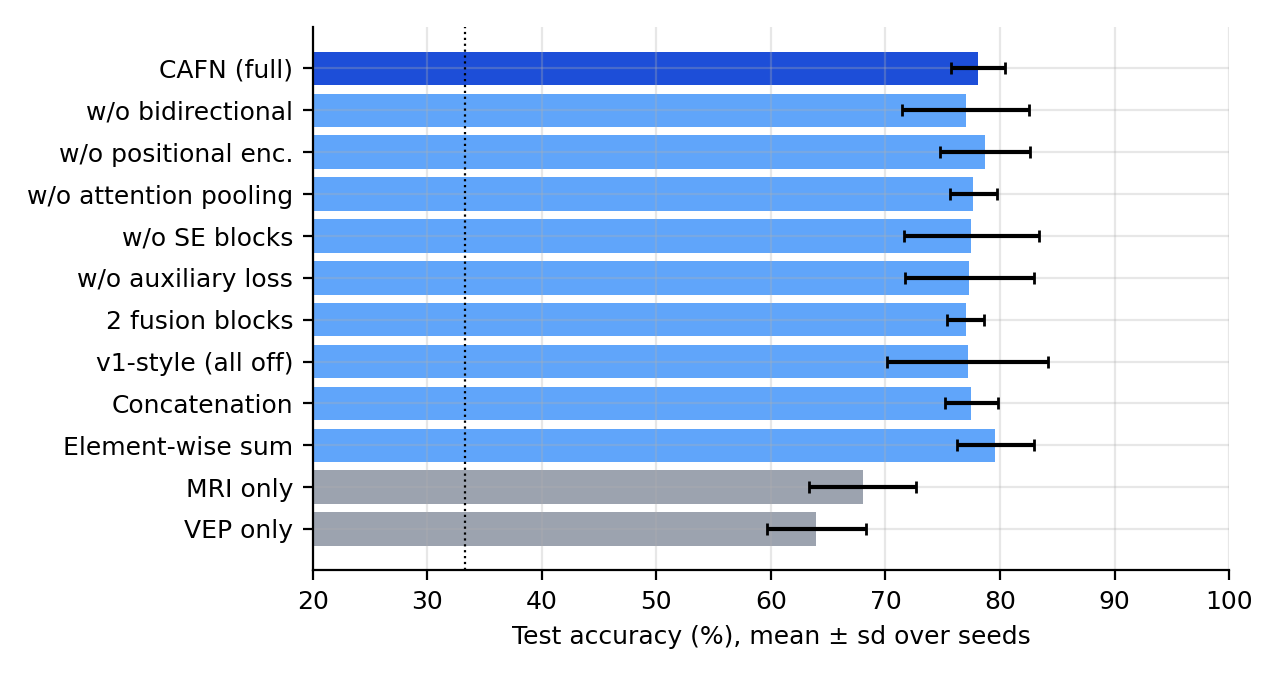
\includegraphics[width=\columnwidth]{results_assets/fig_ablation.png}
\caption{Study A: test accuracy by configuration (bars: mean, whiskers: SD over seeds; dotted line: chance). Grey: unimodal references.}
\label{fig:ablation}
\end{figure}

\subsection{Study A: how informative must each modality be?}
Fig.~\ref{fig:sweep} varies $\mu_{\mathrm{VEP}}$ with the MRI fixed ($n{=}2$ seeds per point; four methods). The VEP-only model rises from chance (45\%) to 97\% while the MRI-only model stays at 63--70\%. The gain of the fused models over the better single modality is largest at intermediate informativeness and vanishes when one modality dominates: +5 points (CAFN) and +7 (concatenation) at $\mu_{\mathrm{VEP}}{=}0.15$, +13 points (CAFN) and +12 (concatenation) at $\mu_{\mathrm{VEP}}{=}0.3$, +5 points (CAFN) and +5 (concatenation) at $\mu_{\mathrm{VEP}}{=}0.5$, +1 points (CAFN) and +2 (concatenation) at $\mu_{\mathrm{VEP}}{=}1$. Fusion therefore never hurt here, helps when both streams carry independent evidence, and converges to the dominant stream otherwise; CAFN and concatenation track each other throughout. With only 2 seeds per point the intervals are wide and the curves should be read as a trend, not as precise estimates.

\begin{figure}[!t]
\centering
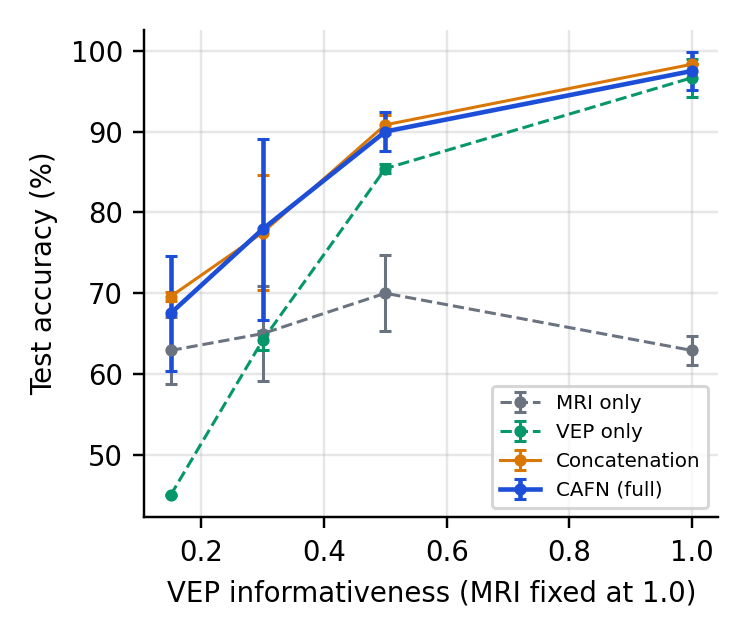
\includegraphics[width=0.78\columnwidth]{results_assets/fig_sweep.png}
\caption{Study A sweep: test accuracy versus VEP informativeness (MRI fixed at 1.0). Dashed: unimodal models; solid: fusion models.}
\label{fig:sweep}
\end{figure}
